\lstset{language=Java, numbers=left, numberstyle=\tiny, stepnumber=2, numbersep=5pt}
\chapter{Introduction}
\label{intro}
In today's world, where increasingly large amounts of data have to be processed and exchanged by distributed systems, the requirements for communication between distributed systems are becoming more and more complex. Not only performance is a problem, but also the requirement to make the services of the distributed systems available to several users at the same time. In other words, every system that is part of the architecture of a distributed system must be able to communicate with every other subsystem at the same time.\\
There are several technologies in the Java environment that can be used for communication within such a distributed system. The most basic variant is the use of Java Sockets. But this assignment favors the Java Remote Method Invocation. This report considers both technologies and presents a possible solution for a distributed system in which both of them play a role.
%%%%%%%%%%%%%%%%%%%%%%%%%%%%%%%%%%%%%%%%%%%%%%%%%%%%%%%%%%%%%%%%%%%%%%%%%%%%%%%%%%%%%%%%%%%%%%%%%%%%%%%%%
%%%%%%%%%%%%%%%%%%%%%%%%%%%%%%%%%%%%%%%%%%%%%%%%%%%%%%%%%%%%%%%%%%%%%%%%%%%%%%%%%%%%%%%%%%%%%%%%%%%%%%%%%
%%%%%%%%%%%%%%%%%%%%%%%%%%%%%%%%%%%%%%%%%%%%%%%%%%%%%%%%%%%%%%%%%%%%%%%%%%%%%%%%%%%%%%%%%%%%%%%%%%%%%%%%%
\chapter{Network Programming in Java}
\label{network-programming}
This chapter explains the theoretical basis for this assignment. The first section focuses on Java sockets, while the second deals with Remote Method Invocation (RMI). The aim is to highlight the differences as well as the advantages and disadvantages of both technologies.
\section{Sockets in Java}
A socket is an endpoint of a bi-directional communication connection between two programs running in different processes on the same computer or on different computers in a network . One socket takes on the role of the server, while the second socket acts as a client. Socket classes are used in Java to represent the connection between a client program and a server program. Sockets provide a simple API and require a hostname and a free port number to be initialized. If two or more sockets are running on the same computer, the hostnames and portnumbers must be different. Before the two processes (no matter if they are running on different computers or not) can communicate with each other, the client and server sockets must perform two different tasks.
\\
First of all, the client must know the hostname and port number of the server in order to connect to it. How exactly this is done depends on the programmer's decision. The server's address data can be stored permanently in the client's program code or can be retrieved by other techniques such as DNS. When establishing a connection between client and server, the client must also identify itself by sending its own host address to the server. The only thing the server has to do is to listen to possible clients attempting to open a connection.
\\
After the connection has been established, data can be transferred in both directions between server and client. The next two chapters show two different socket types and their differences.
\subsection{TCP Socket}
In general there are two different socket types. The first is the \textbf{Stream Socket} whose communication is based on the Transmission Control Protocol (\textbf{TCP}).
\begin{figure}[H]
	\centering
	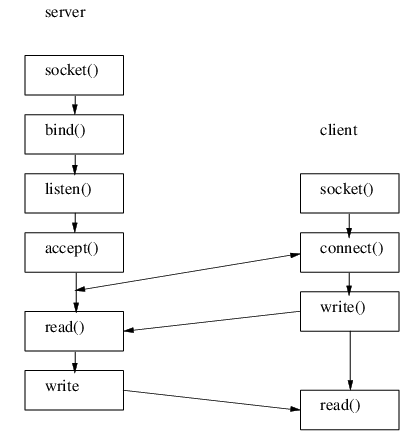
\includegraphics[width =0.7\textwidth]{tcpsocket.PNG}
	\caption{TCP communication between server and client}
	\label{Wallet}
\end{figure}
\section{Java Remote Method Invocation}
%%%%%%%%%%%%%%%%%%%%%%%%%%%%%%%%%%%%%%%%%%%%%%%%%%%%%%%%%%%%%%%%%%%%%%%%%%%%%%%%%%%%%%%%%%%%%%%%%%%%%%%%%
%%%%%%%%%%%%%%%%%%%%%%%%%%%%%%%%%%%%%%%%%%%%%%%%%%%%%%%%%%%%%%%%%%%%%%%%%%%%%%%%%%%%%%%%%%%%%%%%%%%%%%%%%
%%%%%%%%%%%%%%%%%%%%%%%%%%%%%%%%%%%%%%%%%%%%%%%%%%%%%%%%%%%%%%%%%%%%%%%%%%%%%%%%%%%%%%%%%%%%%%%%%%%%%%%%%
\chapter{Job Server/Client Architecture}
\label{job}
\section{Overall Architecture}
\section{UDP-Multicast}
\section{The Job Server}
\section{The Job Client}
\section{Workload-Balancing}
%%%%%%%%%%%%%%%%%%%%%%%%%%%%%%%%%%%%%%%%%%%%%%%%%%%%%%%%%%%%%%%%%%%%%%%%%%%%%%%%%%%%%%%%%%%%%%%%%%%%%%%%%
%%%%%%%%%%%%%%%%%%%%%%%%%%%%%%%%%%%%%%%%%%%%%%%%%%%%%%%%%%%%%%%%%%%%%%%%%%%%%%%%%%%%%%%%%%%%%%%%%%%%%%%%%
%%%%%%%%%%%%%%%%%%%%%%%%%%%%%%%%%%%%%%%%%%%%%%%%%%%%%%%%%%%%%%%%%%%%%%%%%%%%%%%%%%%%%%%%%%%%%%%%%%%%%%%%%
\chapter{Other possible solutions}
\label{other-solutions}
\section{Server Broadcast}
\section{Workload Balancer}

%%%%%%%%%%%%%%%%%%%%%%%%%%%%%%%%%%%%%%%%%%%%%%%%%%%%%%%%%%%%%%%%%%%%%%%%%%%%%%%%%%%%%%%%%%%%%%%%%%%%%%%%%
%%%%%%%%%%%%%%%%%%%%%%%%%%%%%%%%%%%%%%%%%%%%%%%%%%%%%%%%%%%%%%%%%%%%%%%%%%%%%%%%%%%%%%%%%%%%%%%%%%%%%%%%%
%%%%%%%%%%%%%%%%%%%%%%%%%%%%%%%%%%%%%%%%%%%%%%%%%%%%%%%%%%%%%%%%%%%%%%%%%%%%%%%%%%%%%%%%%%%%%%%%%%%%%%%%%
\chapter{Conclusion}
\label{conclusion}
